% Generated by pysimcount.pfchilds -- do not edit; regenerate instead.
% figure: main-cnot-all-formulas -- Every formula, X-Y-Z grouping, cnot gates vs n (cf. Childs et al. 2018 Fig. 3 right)
% source: ../np-main/aggregate.json + ../np-main-n9/seed{seed}, ../np-main-n11/seed{seed} (seeds [1, 2, 3, 4, 5, 6, 7, 8, 9, 10]); run commits: 01d3c275ceae2840002bd1aaea68f59b987c4975, e42ff29056ad9ea7fc7c9899fab334903e42e3e3
% metric=cnot kind=xyz merged (cz, simcount template)
% measured n: mean over seeds of the run's totals; bars min..max over seeds
% r from per-seed power-law fits (n = 5--11), mean count over seeds; r = ceil(a n^b); point=seed-mean; bars = min..max of per-seed fits
% per-step counts exactly affine in n (checked on n = [10, 20, 40], direct build at n = [100])
% shown: suzuki4, suzuki6, mo-q6, mo-q14, bm-q10, mo-o8-q21, morales-y8m10, morales-m8
% removed (see main-cnot-all-formulas-ranking.md): lie-trotter, suzuki2, suzuki8
% figure made at git_commit=e5d9ee696f892e28aced765585653760f8a427c4 git_dirty=False
% derived: main-cnot-all-formulas.tex with zoomed insets by pysimcount.figinset; coordinates copied unchanged; error bars removed on the main axis (insets keep them); source_sha256=49d1738e03ddd55191b52d06eb3dda45f096ccf91d084f3d7f99e65dc13fc6ca
% inset measured: n = 3.7..12, y = 3400..130000; points outside the y-range, not shown in this inset: none
% inset large: n = 170..570, y = 2e+07..3e+09; points outside the y-range, not shown in this inset: none
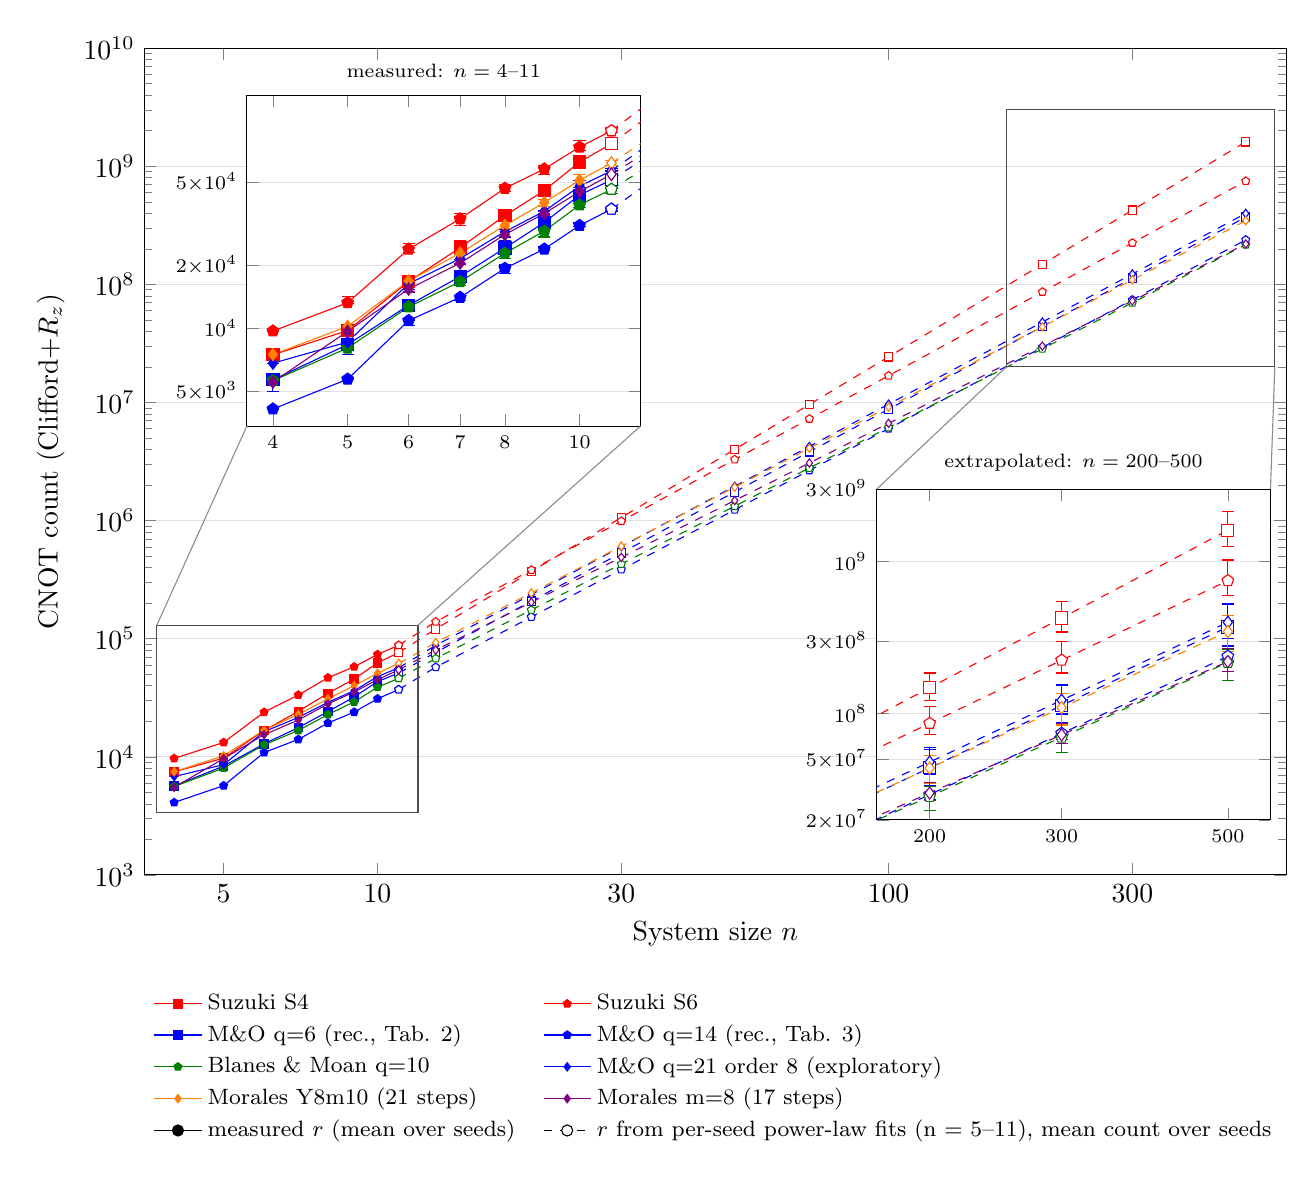
\begin{tikzpicture}
  \begin{loglogaxis}[
    name=main, scale only axis,
    width=14.5cm, height=10.5cm,
    xlabel={System size $n$},
    ylabel={CNOT count (Clifford+$R_z$)},
    xtick={5,10,30,100,300}, xticklabels={5,10,30,100,300},
    xmin=3.5, xmax=600, ymin=1000, ymax=1e+10,
    ymajorgrids=true, grid style={black!12},
    legend style={at={(0.5,-0.13)}, anchor=north, draw=none, font=\footnotesize,
      legend columns=2, /tikz/every even column/.append style={column sep=8pt}},
    legend cell align=left,
  ]
    % suzuki4: measured n, mean over seeds, bars min..max over seeds
    \addplot[red, solid, mark=square*, mark size=1.5pt, mark options={solid, fill=red}] coordinates {
      (4,7459.2)
      (5,9744)
      (6,16707.6)
      (7,24284.4)
      (8,34540.8)
      (9,45549)
      (10,62412)
      (11,76230)
    };
    \addlegendentry{Suzuki S4}
    % suzuki4: extrapolated, r = ceil(3.65267 n^1.59931), per step = 42 n + 0; bars min..max of per-seed fits
    \addplot[red, dashed, mark=square*, mark size=1.5pt, mark options={solid, fill=white}, forget plot] coordinates {
      (11,76230)
      (13,120830)
      (20,370020)
      (30,1.06155e+06)
      (50,4.00848e+06)
      (70,9.61968e+06)
      (100,2.43394e+07)
      (200,1.47922e+08)
      (300,4.25239e+08)
      (500,1.60899e+09)
    };
    % suzuki6: measured n, mean over seeds, bars min..max over seeds
    \addplot[red, solid, mark=pentagon*, mark size=1.5pt, mark options={solid, fill=red}] coordinates {
      (4,9696)
      (5,13231)
      (6,23876.4)
      (7,33370.4)
      (8,46702.4)
      (9,57812.4)
      (10,73528)
      (11,87991.2)
    };
    \addlegendentry{Suzuki S6}
    % suzuki6: extrapolated, r = ceil(1.63295 n^1.35284), per step = 202 n + 0; bars min..max of per-seed fits
    \addplot[red, dashed, mark=pentagon*, mark size=1.5pt, mark options={solid, fill=white}, forget plot] coordinates {
      (11,87991.2)
      (13,139178)
      (20,381780)
      (30,989598)
      (50,3.2926e+06)
      (70,7.26796e+06)
      (100,1.68428e+07)
      (200,8.62823e+07)
      (300,2.24481e+08)
      (500,7.49087e+08)
    };
    % mo-q6: measured n, mean over seeds, bars min..max over seeds
    \addplot[blue, solid, mark=square*, mark size=1.5pt, mark options={solid, fill=blue}] coordinates {
      (4,5660)
      (5,8350)
      (6,12870)
      (7,17675)
      (8,24160)
      (9,32085)
      (10,43300)
      (11,51260)
    };
    \addlegendentry{M\&O q=6 (rec., Tab. 2)}
    % mo-q6: extrapolated, r = ceil(3.93927 n^1.32338), per step = 50 n + 0; bars min..max of per-seed fits
    \addplot[blue, dashed, mark=square*, mark size=1.5pt, mark options={solid, fill=white}, forget plot] coordinates {
      (11,51260)
      (13,76505)
      (20,207900)
      (30,533100)
      (50,1.74725e+06)
      (70,3.82165e+06)
      (100,8.761e+06)
      (200,4.3965e+07)
      (300,1.13001e+08)
      (500,3.71342e+08)
    };
    % mo-q14: measured n, mean over seeds, bars min..max over seeds
    \addplot[blue, solid, mark=pentagon*, mark size=1.5pt, mark options={solid, fill=blue}] coordinates {
      (4,4104)
      (5,5700)
      (6,10875.6)
      (7,14044.8)
      (8,19334.4)
      (9,23905.8)
      (10,31008)
      (11,37118.4)
    };
    \addlegendentry{M\&O q=14 (rec., Tab. 3)}
    % mo-q14: extrapolated, r = ceil(1.412 n^1.28559), per step = 114 n + 0; bars min..max of per-seed fits
    \addplot[blue, dashed, mark=pentagon*, mark size=1.5pt, mark options={solid, fill=white}, forget plot] coordinates {
      (11,37118.4)
      (13,57353.4)
      (20,152760)
      (30,384750)
      (50,1.23348e+06)
      (70,2.65973e+06)
      (100,6.00438e+06)
      (200,2.92889e+07)
      (300,7.40054e+07)
      (500,2.37981e+08)
    };
    % bm-q10: measured n, mean over seeds, bars min..max over seeds
    \addplot[green!50!black, solid, mark=pentagon*, mark size=1.5pt, mark options={solid, fill=green!50!black}] coordinates {
      (4,5608.8)
      (5,8036)
      (6,12644.4)
      (7,16703.4)
      (8,22828.8)
      (9,29151)
      (10,38868)
      (11,46182.4)
    };
    \addlegendentry{Blanes \& Moan q=10}
    % bm-q10: extrapolated, r = ceil(2.82314 n^1.2111), per step = 82 n + 0; bars min..max of per-seed fits
    \addplot[green!50!black, dashed, mark=pentagon*, mark size=1.5pt, mark options={solid, fill=white}, forget plot] coordinates {
      (11,46182.4)
      (13,67904.2)
      (20,175152)
      (30,428532)
      (50,1.32553e+06)
      (70,2.78964e+06)
      (100,6.1418e+06)
      (200,2.84934e+07)
      (300,6.99427e+07)
      (500,2.16874e+08)
    };
    % mo-o8-q21: measured n, mean over seeds, bars min..max over seeds
    \addplot[blue, solid, mark=diamond*, mark size=1.5pt, mark options={solid, fill=blue}] coordinates {
      (4,6800)
      (5,8585)
      (6,16320)
      (7,21539)
      (8,28968)
      (9,36261)
      (10,47770)
      (11,56661)
    };
    \addlegendentry{M\&O q=21 order 8 (exploratory)}
    % mo-o8-q21: extrapolated, r = ceil(1.3736 n^1.30758), per step = 170 n + 0; bars min..max of per-seed fits
    \addplot[blue, dashed, mark=diamond*, mark size=1.5pt, mark options={solid, fill=white}, forget plot] coordinates {
      (11,56661)
      (13,87737)
      (20,236300)
      (30,601290)
      (50,1.95245e+06)
      (70,4.24235e+06)
      (100,9.6662e+06)
      (200,4.79366e+07)
      (300,1.22364e+08)
      (500,3.98548e+08)
    };
    % morales-y8m10: measured n, mean over seeds, bars min..max over seeds
    \addplot[orange, solid, mark=diamond*, mark size=1.5pt, mark options={solid, fill=orange}] coordinates {
      (4,7480)
      (5,10200)
      (6,16830)
      (7,22848)
      (8,31008)
      (9,39933)
      (10,51000)
      (11,61710)
    };
    \addlegendentry{Morales Y8m10 (21 steps)}
    % morales-y8m10: extrapolated, r = ceil(1.66328 n^1.25438), per step = 170 n + 0; bars min..max of per-seed fits
    \addplot[orange, dashed, mark=diamond*, mark size=1.5pt, mark options={solid, fill=white}, forget plot] coordinates {
      (11,61710)
      (13,92599)
      (20,244120)
      (30,607410)
      (50,1.9176e+06)
      (70,4.09836e+06)
      (100,9.1596e+06)
      (200,4.3758e+07)
      (300,1.09303e+08)
      (500,3.46477e+08)
    };
    % morales-m8: measured n, mean over seeds, bars min..max over seeds
    \addplot[violet, solid, mark=diamond*, mark size=1.5pt, mark options={solid, fill=violet}] coordinates {
      (4,5520)
      (5,9660)
      (6,15400.8)
      (7,20479.2)
      (8,28041.6)
      (9,35397)
      (10,44988)
      (11,54496.2)
    };
    \addlegendentry{Morales m=8 (17 steps)}
    % morales-m8: extrapolated, r = ceil(2.19247 n^1.17079), per step = 138 n + 0; bars min..max of per-seed fits
    \addplot[violet, dashed, mark=diamond*, mark size=1.5pt, mark options={solid, fill=white}, forget plot] coordinates {
      (11,54496.2)
      (13,80191.8)
      (20,203136)
      (30,488934)
      (50,1.47936e+06)
      (70,3.07188e+06)
      (100,6.66264e+06)
      (200,3.0026e+07)
      (300,7.24417e+07)
      (500,2.19834e+08)
    };
    \addlegendimage{black, solid, mark=*, mark options={solid, fill=black}}
    \addlegendentry{measured $r$ (mean over seeds)}
    \addlegendimage{black, dashed, mark=*, mark options={solid, fill=white}}
    \addlegendentry{$r$ from per-seed power-law fits (n = 5--11), mean count over seeds}
    % zoom window of inset measured
    \draw[black!70] (axis cs:3.7,3400) rectangle (axis cs:12,130000);
    \coordinate (zoom-measured-sw) at (axis cs:3.7,3400);
    \coordinate (zoom-measured-nw) at (axis cs:3.7,130000);
    \coordinate (zoom-measured-se) at (axis cs:12,3400);
    \coordinate (zoom-measured-ne) at (axis cs:12,130000);
    % zoom window of inset large
    \draw[black!70] (axis cs:170,2e+07) rectangle (axis cs:570,3e+09);
    \coordinate (zoom-large-sw) at (axis cs:170,2e+07);
    \coordinate (zoom-large-nw) at (axis cs:170,3e+09);
    \coordinate (zoom-large-se) at (axis cs:570,2e+07);
    \coordinate (zoom-large-ne) at (axis cs:570,3e+09);
  \end{loglogaxis}
  \begin{loglogaxis}[
    name=inset-measured, scale only axis,
    at={(main.south west)}, anchor=south west, xshift=1.3cm, yshift=5.7cm,
    width=5.0cm, height=4.2cm,
    xmin=3.7, xmax=12, ymin=3400, ymax=130000,
    xtick={4,5,6,7,8,10}, xticklabels={4,5,6,7,8,10},
    ytick={5000,10000,20000,50000}, yticklabels={$5{\times}10^{3}$,$10^{4}$,$2{\times}10^{4}$,$5{\times}10^{4}$},
    minor tick num=0, xminorticks=false, yminorticks=false,
    ymajorgrids=true, grid style={black!12},
    tick label style={font=\scriptsize},
    axis background/.style={fill=white},
    title={measured: $n = 4$--$11$}, title style={font=\scriptsize, yshift=-3pt},
  ]
    \addplot[red, solid, mark=square*, mark size=2.2pt, mark options={solid, fill=red}, forget plot, error bars/.cd, y dir=both, y explicit, error bar style={solid}] coordinates {
      (4,7459.2) += (0,100.8) -= (0,67.2)
      (5,9744) += (0,336) -= (0,294)
      (6,16707.6) += (0,1184.4) -= (0,831.6)
      (7,24284.4) += (0,1881.6) -= (0,1646.4)
      (8,34540.8) += (0,1411.2) -= (0,1276.8)
      (9,45549) += (0,2079) -= (0,2457)
      (10,62412) += (0,4788) -= (0,2352)
      (11,76230) += (0,3234) -= (0,1848)
    };
    \addplot[red, dashed, mark=square*, mark size=2.2pt, mark options={solid, fill=white}, forget plot, error bars/.cd, y dir=both, y explicit, error bar style={solid}] coordinates {
      (11,76230)
      (13,120830) += (0,5296.2) -= (0,3985.8)
      (20,370020) += (0,27300) -= (0,20580)
      (30,1.06155e+06) += (0,108990) -= (0,81270)
      (50,4.00848e+06) += (0,567420) -= (0,411180)
      (70,9.61968e+06) += (0,1.61112e+06) -= (0,1.14954e+06)
      (100,2.43394e+07) += (0,4.75398e+06) -= (0,3.34362e+06)
      (200,1.47922e+08) += (0,3.70709e+07) -= (0,2.53495e+07)
      (300,4.25239e+08) += (0,1.20644e+08) -= (0,8.11705e+07)
      (500,1.60899e+09) += (0,5.24758e+08) -= (0,3.46154e+08)
    };
    \addplot[red, solid, mark=pentagon*, mark size=2.2pt, mark options={solid, fill=red}, forget plot, error bars/.cd, y dir=both, y explicit, error bar style={solid}] coordinates {
      (4,9696) += (0,0) -= (0,0)
      (5,13231) += (0,909) -= (0,101)
      (6,23876.4) += (0,1575.6) -= (0,848.4)
      (7,33370.4) += (0,1979.6) -= (0,2262.4)
      (8,46702.4) += (0,1777.6) -= (0,1454.4)
      (9,57812.4) += (0,2181.6) -= (0,3272.4)
      (10,73528) += (0,5252) -= (0,2828)
      (11,87991.2) += (0,3110.8) -= (0,1333.2)
    };
    \addplot[red, dashed, mark=pentagon*, mark size=2.2pt, mark options={solid, fill=white}, forget plot, error bars/.cd, y dir=both, y explicit, error bar style={solid}] coordinates {
      (11,87991.2)
      (13,139178) += (0,7878) -= (0,2626)
      (20,381780) += (0,30300) -= (0,14140)
      (30,989598) += (0,113322) -= (0,56358)
      (50,3.2926e+06) += (0,525200) -= (0,282800)
      (70,7.26796e+06) += (0,1.37158e+06) -= (0,749420)
      (100,1.68428e+07) += (0,3.70064e+06) -= (0,2.03616e+06)
      (200,8.62823e+07) += (0,2.43733e+07) -= (0,1.34411e+07)
      (300,2.24481e+08) += (0,7.17928e+07) -= (0,3.94688e+07)
      (500,7.49087e+08) += (0,2.75659e+08) -= (0,1.50258e+08)
    };
    \addplot[blue, solid, mark=square*, mark size=2.2pt, mark options={solid, fill=blue}, forget plot, error bars/.cd, y dir=both, y explicit, error bar style={solid}] coordinates {
      (4,5660) += (0,340) -= (0,660)
      (5,8350) += (0,400) -= (0,850)
      (6,12870) += (0,330) -= (0,570)
      (7,17675) += (0,875) -= (0,1225)
      (8,24160) += (0,2240) -= (0,1360)
      (9,32085) += (0,1665) -= (0,2385)
      (10,43300) += (0,1700) -= (0,2800)
      (11,51260) += (0,5390) -= (0,4510)
    };
    \addplot[blue, dashed, mark=square*, mark size=2.2pt, mark options={solid, fill=white}, forget plot, error bars/.cd, y dir=both, y explicit, error bar style={solid}] coordinates {
      (11,51260)
      (13,76505) += (0,4745) -= (0,3055)
      (20,207900) += (0,21100) -= (0,12900)
      (30,533100) += (0,72900) -= (0,48600)
      (50,1.74725e+06) += (0,320250) -= (0,214750)
      (70,3.82165e+06) += (0,815850) -= (0,545650)
      (100,8.761e+06) += (0,2.164e+06) -= (0,1.441e+06)
      (200,4.3965e+07) += (0,1.3765e+07) -= (0,9.035e+06)
      (300,1.13001e+08) += (0,3.9894e+07) -= (0,2.5851e+07)
      (500,3.71342e+08) += (0,1.50232e+08) -= (0,9.55425e+07)
    };
    \addplot[blue, solid, mark=pentagon*, mark size=2.2pt, mark options={solid, fill=blue}, forget plot, error bars/.cd, y dir=both, y explicit, error bar style={solid}] coordinates {
      (4,4104) += (0,0) -= (0,0)
      (5,5700) += (0,0) -= (0,0)
      (6,10875.6) += (0,68.4) -= (0,615.6)
      (7,14044.8) += (0,319.2) -= (0,478.8)
      (8,19334.4) += (0,729.6) -= (0,1094.4)
      (9,23905.8) += (0,718.2) -= (0,307.8)
      (10,31008) += (0,912) -= (0,228)
      (11,37118.4) += (0,501.6) -= (0,752.4)
    };
    \addplot[blue, dashed, mark=pentagon*, mark size=2.2pt, mark options={solid, fill=white}, forget plot, error bars/.cd, y dir=both, y explicit, error bar style={solid}] coordinates {
      (11,37118.4)
      (13,57353.4) += (0,444.6) -= (0,1037.4)
      (20,152760) += (0,4560) -= (0,4560)
      (30,384750) += (0,18810) -= (0,15390)
      (50,1.23348e+06) += (0,88920) -= (0,59280)
      (70,2.65973e+06) += (0,237006) -= (0,146034)
      (100,6.00438e+06) += (0,641820) -= (0,361380)
      (200,2.92889e+07) += (0,4.09032e+06) -= (0,2.15688e+06)
      (300,7.40054e+07) += (0,1.18366e+07) -= (0,6.04998e+06)
      (500,2.37981e+08) += (0,4.40553e+07) -= (0,2.17797e+07)
    };
    \addplot[green!50!black, solid, mark=pentagon*, mark size=2.2pt, mark options={solid, fill=green!50!black}, forget plot, error bars/.cd, y dir=both, y explicit, error bar style={solid}] coordinates {
      (4,5608.8) += (0,295.2) -= (0,32.8)
      (5,8036) += (0,164) -= (0,246)
      (6,12644.4) += (0,147.6) -= (0,344.4)
      (7,16703.4) += (0,516.6) -= (0,631.4)
      (8,22828.8) += (0,1443.2) -= (0,1180.8)
      (9,29151) += (0,1107) -= (0,1845)
      (10,38868) += (0,492) -= (0,1148)
      (11,46182.4) += (0,2525.6) -= (0,1984.4)
    };
    \addplot[green!50!black, dashed, mark=pentagon*, mark size=2.2pt, mark options={solid, fill=white}, forget plot, error bars/.cd, y dir=both, y explicit, error bar style={solid}] coordinates {
      (11,46182.4)
      (13,67904.2) += (0,1385.8) -= (0,1812.2)
      (20,175152) += (0,6888) -= (0,9512)
      (30,428532) += (0,26568) -= (0,34932)
      (50,1.32553e+06) += (0,121770) -= (0,144730)
      (70,2.78964e+06) += (0,304220) -= (0,361620)
      (100,6.1418e+06) += (0,795400) -= (0,918400)
      (200,2.84934e+07) += (0,4.83144e+06) -= (0,5.33656e+06)
      (300,6.99427e+07) += (0,1.34759e+07) -= (0,1.45927e+07)
      (500,2.16874e+08) += (0,4.82324e+07) -= (0,5.09876e+07)
    };
    \addplot[blue, solid, mark=diamond*, mark size=2.2pt, mark options={solid, fill=blue}, forget plot, error bars/.cd, y dir=both, y explicit, error bar style={solid}] coordinates {
      (4,6800) += (0,0) -= (0,0)
      (5,8585) += (0,765) -= (0,85)
      (6,16320) += (0,1020) -= (0,1020)
      (7,21539) += (0,1071) -= (0,1309)
      (8,28968) += (0,952) -= (0,1768)
      (9,36261) += (0,459) -= (0,1071)
      (10,47770) += (0,3230) -= (0,1870)
      (11,56661) += (0,1309) -= (0,561)
    };
    \addplot[blue, dashed, mark=diamond*, mark size=2.2pt, mark options={solid, fill=white}, forget plot, error bars/.cd, y dir=both, y explicit, error bar style={solid}] coordinates {
      (11,56661)
      (13,87737) += (0,2873) -= (0,1547)
      (20,236300) += (0,15300) -= (0,8500)
      (30,601290) += (0,51510) -= (0,35190)
      (50,1.95245e+06) += (0,249050) -= (0,175950)
      (70,4.24235e+06) += (0,660450) -= (0,458150)
      (100,9.6662e+06) += (0,1.7918e+06) -= (0,1.2512e+06)
      (200,4.79366e+07) += (0,1.16314e+07) -= (0,8.0206e+06)
      (300,1.22364e+08) += (0,3.39507e+07) -= (0,2.30673e+07)
      (500,3.98548e+08) += (0,1.28537e+08) -= (0,8.5833e+07)
    };
    \addplot[orange, solid, mark=diamond*, mark size=2.2pt, mark options={solid, fill=orange}, forget plot, error bars/.cd, y dir=both, y explicit, error bar style={solid}] coordinates {
      (4,7480) += (0,0) -= (0,0)
      (5,10200) += (0,0) -= (0,0)
      (6,16830) += (0,510) -= (0,510)
      (7,22848) += (0,952) -= (0,238)
      (8,31008) += (0,1632) -= (0,1088)
      (9,39933) += (0,1377) -= (0,1683)
      (10,51000) += (0,3400) -= (0,1700)
      (11,61710) += (0,1870) -= (0,1870)
    };
    \addplot[orange, dashed, mark=diamond*, mark size=2.2pt, mark options={solid, fill=white}, forget plot, error bars/.cd, y dir=both, y explicit, error bar style={solid}] coordinates {
      (11,61710)
      (13,92599) += (0,2431) -= (0,4199)
      (20,244120) += (0,14280) -= (0,16320)
      (30,607410) += (0,55590) -= (0,56610)
      (50,1.9176e+06) += (0,232900) -= (0,243100)
      (70,4.09836e+06) += (0,590240) -= (0,599760)
      (100,9.1596e+06) += (0,1.5504e+06) -= (0,1.5436e+06)
      (200,4.3758e+07) += (0,9.554e+06) -= (0,9.112e+06)
      (300,1.09303e+08) += (0,2.70198e+07) -= (0,2.52552e+07)
      (500,3.46477e+08) += (0,9.8413e+07) -= (0,8.9862e+07)
    };
    \addplot[violet, solid, mark=diamond*, mark size=2.2pt, mark options={solid, fill=violet}, forget plot, error bars/.cd, y dir=both, y explicit, error bar style={solid}] coordinates {
      (4,5520) += (0,0) -= (0,0)
      (5,9660) += (0,0) -= (0,0)
      (6,15400.8) += (0,331.2) -= (0,496.8)
      (7,20479.2) += (0,772.8) -= (0,193.2)
      (8,28041.6) += (0,1766.4) -= (0,441.6)
      (9,35397) += (0,621) -= (0,621)
      (10,44988) += (0,1932) -= (0,828)
      (11,54496.2) += (0,1669.8) -= (0,1366.2)
    };
    \addplot[violet, dashed, mark=diamond*, mark size=2.2pt, mark options={solid, fill=white}, forget plot, error bars/.cd, y dir=both, y explicit, error bar style={solid}] coordinates {
      (11,54496.2)
      (13,80191.8) += (0,2332.2) -= (0,1255.8)
      (20,203136) += (0,9384) -= (0,7176)
      (30,488934) += (0,32706) -= (0,25254)
      (50,1.47936e+06) += (0,142140) -= (0,99360)
      (70,3.07188e+06) += (0,338100) -= (0,231840)
      (100,6.66264e+06) += (0,872160) -= (0,590640)
      (200,3.0026e+07) += (0,5.02596e+06) -= (0,3.30924e+06)
      (300,7.24417e+07) += (0,1.37117e+07) -= (0,8.89272e+06)
      (500,2.19834e+08) += (0,4.7817e+07) -= (0,3.0498e+07)
    };
  \end{loglogaxis}
  \draw[black!45] (zoom-measured-nw) -- (inset-measured.south west);
  \draw[black!45] (zoom-measured-ne) -- (inset-measured.south east);
  \begin{loglogaxis}[
    name=inset-large, scale only axis,
    at={(main.south west)}, anchor=south west, xshift=9.3cm, yshift=0.7cm,
    width=5.0cm, height=4.2cm,
    xmin=170, xmax=570, ymin=2e+07, ymax=3e+09,
    xtick={200,300,500}, xticklabels={200,300,500},
    ytick={2e+07,5e+07,1e+08,3e+08,1e+09,3e+09}, yticklabels={$2{\times}10^{7}$,$5{\times}10^{7}$,$10^{8}$,$3{\times}10^{8}$,$10^{9}$,$3{\times}10^{9}$},
    minor tick num=0, xminorticks=false, yminorticks=false,
    ymajorgrids=true, grid style={black!12},
    tick label style={font=\scriptsize},
    axis background/.style={fill=white},
    title={extrapolated: $n = 200$--$500$}, title style={font=\scriptsize, yshift=-3pt},
  ]
    \addplot[red, solid, mark=square*, mark size=2.2pt, mark options={solid, fill=red}, forget plot, error bars/.cd, y dir=both, y explicit, error bar style={solid}] coordinates {
      (4,7459.2) += (0,100.8) -= (0,67.2)
      (5,9744) += (0,336) -= (0,294)
      (6,16707.6) += (0,1184.4) -= (0,831.6)
      (7,24284.4) += (0,1881.6) -= (0,1646.4)
      (8,34540.8) += (0,1411.2) -= (0,1276.8)
      (9,45549) += (0,2079) -= (0,2457)
      (10,62412) += (0,4788) -= (0,2352)
      (11,76230) += (0,3234) -= (0,1848)
    };
    \addplot[red, dashed, mark=square*, mark size=2.2pt, mark options={solid, fill=white}, forget plot, error bars/.cd, y dir=both, y explicit, error bar style={solid}] coordinates {
      (11,76230)
      (13,120830) += (0,5296.2) -= (0,3985.8)
      (20,370020) += (0,27300) -= (0,20580)
      (30,1.06155e+06) += (0,108990) -= (0,81270)
      (50,4.00848e+06) += (0,567420) -= (0,411180)
      (70,9.61968e+06) += (0,1.61112e+06) -= (0,1.14954e+06)
      (100,2.43394e+07) += (0,4.75398e+06) -= (0,3.34362e+06)
      (200,1.47922e+08) += (0,3.70709e+07) -= (0,2.53495e+07)
      (300,4.25239e+08) += (0,1.20644e+08) -= (0,8.11705e+07)
      (500,1.60899e+09) += (0,5.24758e+08) -= (0,3.46154e+08)
    };
    \addplot[red, solid, mark=pentagon*, mark size=2.2pt, mark options={solid, fill=red}, forget plot, error bars/.cd, y dir=both, y explicit, error bar style={solid}] coordinates {
      (4,9696) += (0,0) -= (0,0)
      (5,13231) += (0,909) -= (0,101)
      (6,23876.4) += (0,1575.6) -= (0,848.4)
      (7,33370.4) += (0,1979.6) -= (0,2262.4)
      (8,46702.4) += (0,1777.6) -= (0,1454.4)
      (9,57812.4) += (0,2181.6) -= (0,3272.4)
      (10,73528) += (0,5252) -= (0,2828)
      (11,87991.2) += (0,3110.8) -= (0,1333.2)
    };
    \addplot[red, dashed, mark=pentagon*, mark size=2.2pt, mark options={solid, fill=white}, forget plot, error bars/.cd, y dir=both, y explicit, error bar style={solid}] coordinates {
      (11,87991.2)
      (13,139178) += (0,7878) -= (0,2626)
      (20,381780) += (0,30300) -= (0,14140)
      (30,989598) += (0,113322) -= (0,56358)
      (50,3.2926e+06) += (0,525200) -= (0,282800)
      (70,7.26796e+06) += (0,1.37158e+06) -= (0,749420)
      (100,1.68428e+07) += (0,3.70064e+06) -= (0,2.03616e+06)
      (200,8.62823e+07) += (0,2.43733e+07) -= (0,1.34411e+07)
      (300,2.24481e+08) += (0,7.17928e+07) -= (0,3.94688e+07)
      (500,7.49087e+08) += (0,2.75659e+08) -= (0,1.50258e+08)
    };
    \addplot[blue, solid, mark=square*, mark size=2.2pt, mark options={solid, fill=blue}, forget plot, error bars/.cd, y dir=both, y explicit, error bar style={solid}] coordinates {
      (4,5660) += (0,340) -= (0,660)
      (5,8350) += (0,400) -= (0,850)
      (6,12870) += (0,330) -= (0,570)
      (7,17675) += (0,875) -= (0,1225)
      (8,24160) += (0,2240) -= (0,1360)
      (9,32085) += (0,1665) -= (0,2385)
      (10,43300) += (0,1700) -= (0,2800)
      (11,51260) += (0,5390) -= (0,4510)
    };
    \addplot[blue, dashed, mark=square*, mark size=2.2pt, mark options={solid, fill=white}, forget plot, error bars/.cd, y dir=both, y explicit, error bar style={solid}] coordinates {
      (11,51260)
      (13,76505) += (0,4745) -= (0,3055)
      (20,207900) += (0,21100) -= (0,12900)
      (30,533100) += (0,72900) -= (0,48600)
      (50,1.74725e+06) += (0,320250) -= (0,214750)
      (70,3.82165e+06) += (0,815850) -= (0,545650)
      (100,8.761e+06) += (0,2.164e+06) -= (0,1.441e+06)
      (200,4.3965e+07) += (0,1.3765e+07) -= (0,9.035e+06)
      (300,1.13001e+08) += (0,3.9894e+07) -= (0,2.5851e+07)
      (500,3.71342e+08) += (0,1.50232e+08) -= (0,9.55425e+07)
    };
    \addplot[blue, solid, mark=pentagon*, mark size=2.2pt, mark options={solid, fill=blue}, forget plot, error bars/.cd, y dir=both, y explicit, error bar style={solid}] coordinates {
      (4,4104) += (0,0) -= (0,0)
      (5,5700) += (0,0) -= (0,0)
      (6,10875.6) += (0,68.4) -= (0,615.6)
      (7,14044.8) += (0,319.2) -= (0,478.8)
      (8,19334.4) += (0,729.6) -= (0,1094.4)
      (9,23905.8) += (0,718.2) -= (0,307.8)
      (10,31008) += (0,912) -= (0,228)
      (11,37118.4) += (0,501.6) -= (0,752.4)
    };
    \addplot[blue, dashed, mark=pentagon*, mark size=2.2pt, mark options={solid, fill=white}, forget plot, error bars/.cd, y dir=both, y explicit, error bar style={solid}] coordinates {
      (11,37118.4)
      (13,57353.4) += (0,444.6) -= (0,1037.4)
      (20,152760) += (0,4560) -= (0,4560)
      (30,384750) += (0,18810) -= (0,15390)
      (50,1.23348e+06) += (0,88920) -= (0,59280)
      (70,2.65973e+06) += (0,237006) -= (0,146034)
      (100,6.00438e+06) += (0,641820) -= (0,361380)
      (200,2.92889e+07) += (0,4.09032e+06) -= (0,2.15688e+06)
      (300,7.40054e+07) += (0,1.18366e+07) -= (0,6.04998e+06)
      (500,2.37981e+08) += (0,4.40553e+07) -= (0,2.17797e+07)
    };
    \addplot[green!50!black, solid, mark=pentagon*, mark size=2.2pt, mark options={solid, fill=green!50!black}, forget plot, error bars/.cd, y dir=both, y explicit, error bar style={solid}] coordinates {
      (4,5608.8) += (0,295.2) -= (0,32.8)
      (5,8036) += (0,164) -= (0,246)
      (6,12644.4) += (0,147.6) -= (0,344.4)
      (7,16703.4) += (0,516.6) -= (0,631.4)
      (8,22828.8) += (0,1443.2) -= (0,1180.8)
      (9,29151) += (0,1107) -= (0,1845)
      (10,38868) += (0,492) -= (0,1148)
      (11,46182.4) += (0,2525.6) -= (0,1984.4)
    };
    \addplot[green!50!black, dashed, mark=pentagon*, mark size=2.2pt, mark options={solid, fill=white}, forget plot, error bars/.cd, y dir=both, y explicit, error bar style={solid}] coordinates {
      (11,46182.4)
      (13,67904.2) += (0,1385.8) -= (0,1812.2)
      (20,175152) += (0,6888) -= (0,9512)
      (30,428532) += (0,26568) -= (0,34932)
      (50,1.32553e+06) += (0,121770) -= (0,144730)
      (70,2.78964e+06) += (0,304220) -= (0,361620)
      (100,6.1418e+06) += (0,795400) -= (0,918400)
      (200,2.84934e+07) += (0,4.83144e+06) -= (0,5.33656e+06)
      (300,6.99427e+07) += (0,1.34759e+07) -= (0,1.45927e+07)
      (500,2.16874e+08) += (0,4.82324e+07) -= (0,5.09876e+07)
    };
    \addplot[blue, solid, mark=diamond*, mark size=2.2pt, mark options={solid, fill=blue}, forget plot, error bars/.cd, y dir=both, y explicit, error bar style={solid}] coordinates {
      (4,6800) += (0,0) -= (0,0)
      (5,8585) += (0,765) -= (0,85)
      (6,16320) += (0,1020) -= (0,1020)
      (7,21539) += (0,1071) -= (0,1309)
      (8,28968) += (0,952) -= (0,1768)
      (9,36261) += (0,459) -= (0,1071)
      (10,47770) += (0,3230) -= (0,1870)
      (11,56661) += (0,1309) -= (0,561)
    };
    \addplot[blue, dashed, mark=diamond*, mark size=2.2pt, mark options={solid, fill=white}, forget plot, error bars/.cd, y dir=both, y explicit, error bar style={solid}] coordinates {
      (11,56661)
      (13,87737) += (0,2873) -= (0,1547)
      (20,236300) += (0,15300) -= (0,8500)
      (30,601290) += (0,51510) -= (0,35190)
      (50,1.95245e+06) += (0,249050) -= (0,175950)
      (70,4.24235e+06) += (0,660450) -= (0,458150)
      (100,9.6662e+06) += (0,1.7918e+06) -= (0,1.2512e+06)
      (200,4.79366e+07) += (0,1.16314e+07) -= (0,8.0206e+06)
      (300,1.22364e+08) += (0,3.39507e+07) -= (0,2.30673e+07)
      (500,3.98548e+08) += (0,1.28537e+08) -= (0,8.5833e+07)
    };
    \addplot[orange, solid, mark=diamond*, mark size=2.2pt, mark options={solid, fill=orange}, forget plot, error bars/.cd, y dir=both, y explicit, error bar style={solid}] coordinates {
      (4,7480) += (0,0) -= (0,0)
      (5,10200) += (0,0) -= (0,0)
      (6,16830) += (0,510) -= (0,510)
      (7,22848) += (0,952) -= (0,238)
      (8,31008) += (0,1632) -= (0,1088)
      (9,39933) += (0,1377) -= (0,1683)
      (10,51000) += (0,3400) -= (0,1700)
      (11,61710) += (0,1870) -= (0,1870)
    };
    \addplot[orange, dashed, mark=diamond*, mark size=2.2pt, mark options={solid, fill=white}, forget plot, error bars/.cd, y dir=both, y explicit, error bar style={solid}] coordinates {
      (11,61710)
      (13,92599) += (0,2431) -= (0,4199)
      (20,244120) += (0,14280) -= (0,16320)
      (30,607410) += (0,55590) -= (0,56610)
      (50,1.9176e+06) += (0,232900) -= (0,243100)
      (70,4.09836e+06) += (0,590240) -= (0,599760)
      (100,9.1596e+06) += (0,1.5504e+06) -= (0,1.5436e+06)
      (200,4.3758e+07) += (0,9.554e+06) -= (0,9.112e+06)
      (300,1.09303e+08) += (0,2.70198e+07) -= (0,2.52552e+07)
      (500,3.46477e+08) += (0,9.8413e+07) -= (0,8.9862e+07)
    };
    \addplot[violet, solid, mark=diamond*, mark size=2.2pt, mark options={solid, fill=violet}, forget plot, error bars/.cd, y dir=both, y explicit, error bar style={solid}] coordinates {
      (4,5520) += (0,0) -= (0,0)
      (5,9660) += (0,0) -= (0,0)
      (6,15400.8) += (0,331.2) -= (0,496.8)
      (7,20479.2) += (0,772.8) -= (0,193.2)
      (8,28041.6) += (0,1766.4) -= (0,441.6)
      (9,35397) += (0,621) -= (0,621)
      (10,44988) += (0,1932) -= (0,828)
      (11,54496.2) += (0,1669.8) -= (0,1366.2)
    };
    \addplot[violet, dashed, mark=diamond*, mark size=2.2pt, mark options={solid, fill=white}, forget plot, error bars/.cd, y dir=both, y explicit, error bar style={solid}] coordinates {
      (11,54496.2)
      (13,80191.8) += (0,2332.2) -= (0,1255.8)
      (20,203136) += (0,9384) -= (0,7176)
      (30,488934) += (0,32706) -= (0,25254)
      (50,1.47936e+06) += (0,142140) -= (0,99360)
      (70,3.07188e+06) += (0,338100) -= (0,231840)
      (100,6.66264e+06) += (0,872160) -= (0,590640)
      (200,3.0026e+07) += (0,5.02596e+06) -= (0,3.30924e+06)
      (300,7.24417e+07) += (0,1.37117e+07) -= (0,8.89272e+06)
      (500,2.19834e+08) += (0,4.7817e+07) -= (0,3.0498e+07)
    };
  \end{loglogaxis}
  \draw[black!45] (zoom-large-sw) -- (inset-large.north west);
  \draw[black!45] (zoom-large-se) -- (inset-large.north east);
\end{tikzpicture}
